
% !TEX encoding = UTF-8 Unicode 
% !TEX root = FieldGuide.tex

\subpart{Zero shape parameters}

\Sec{Uniform Distribution}
\label{sec:Uniform}
The simplest continuous distribution is a uniform density over an interval.

 \dist{Uniform} (flat, rectangular) distribution: 
\begin{align}
\label{Uniform}
\opr{Uniform}(x\given a,s) =& \frac{1}{|s|} 				\checked 
\\
& \text{for } a, s  \text{ in } \mathbb{R}, 				\checked
\notag\\   
\text{ support } & x\in  [a,a+s], \quad s>0  			\checked
\notag \\ 
& x\in    [a+s,a], \quad s<0 \notag					\checked
\end{align}
The uniform distribution is also commonly parameterized with the boundary points, $a$ and $b=a+s$, rather than location $a$ and scale $s$ as here. 
Note that the discrete analog of the continuous uniform distribution is  also often referred to as the uniform distribution.



\SSec{Special cases}
The {\bf standard uniform} distribution covers the unit interval, $x\in[0,1]$.
\begin{align}
\label{StdUniform}
\opr{StdUniform}(x)  = \opr{Uniform}(x\given 0,1) \checked
\end{align}
The {\bf standardized uniform} distribution, with zero mean and unit variance, is $\opr{Uniform}(x\given -\sqrt{3},2\sqrt{3})$.

\phantomsection\addcontentsline{toc}{subsection}{~~~~~~~~~~~~Half uniform}
\phantomsection\addcontentsline{toc}{subsection}{~~~~~~~~~~~~Unbounded uniform}
\phantomsection\addcontentsline{toc}{subsection}{~~~~~~~~~~~~Degenerate}
Three limits of the uniform distribution are important. If one of the boundary points is infinite (infinite scale), then we obtain an improper (unnormalizable) {\bf half-uniform} distribution. In the limit that both boundary points reach infinity (with opposite signs) we obtain an {\bf unbounded uniform} distribution.
In the alternative limit that the boundary points converge, we obtain a {\bf degenerate} (delta, Dirac) \label{Delta} distribution, wherein the entire probability density  is concentrated on a single point.




\SSec{Interrelations}
Uniform distributions, with finite, semi-infinite, or infinite support, are limits of many distribution families. The finite uniform distribution is a special case of the beta distribution \eqref{Beta}.
\begin{align*}
 \opr{Uniform}(x\given a,s)  &=  \opr{Beta}(x\given a, s, 1,1) 	\checked
 \\
 &\qquad=  \opr{CentralBeta}(x\given a+\tfrac{s}{2}, s) \checked
\end{align*}
Similarly, the semi-infinite uniform distribution is a limit of the Pareto \eqref{Pareto}, beta prime \eqref{BetaPrime}, Amoroso \eqref{Amoroso}, gamma \eqref{Gamma}, and exponential  \eqref{Exp} distributions, and the infinite support uniform distribution is a limit of the normal \eqref{Normal}, Cauchy \eqref{Cauchy}, logistic \eqref{Logistic} and  gamma-exponential  \eqref{GammaExp} distributions, among others. 

The order statistics \secref{OrderStatistic} of the uniform distribution is the beta distribution~\eqref{Beta}.
\[
\opr{OrderStatistic}_{\opr{Uniform}(a,s)}(x \given \alpha, \gamma) =  \opr{Beta}(x\given a, s, \alpha, \gamma) 
\checked
\notag
\]


\begin{figure}[t]
\begin{center}
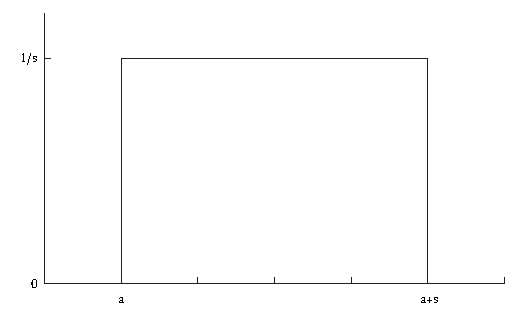
\includegraphics[width=\textwidth]{pdfUniform}
\end{center}
\caption[Uniform distribution]{Uniform distribution, $\opr{Uniform}(x\given a,s)$ \eqref{Uniform}}
\end{figure}


The standard uniform distribution is related to every other continuous distribution via the  inverse probability integral transform (Smirnov transform)\index{Smirnov transform}\index{inverse probability integral transform}. If $X$ is a random variable and $F_X^{-1}(z)$ the inverse of the corresponding cumulative distribution function then 
\[ 
X \sim F_X^{-1}\bigl( \opr{StdUniform}() \bigr) \ .  \checked
\notag
\]
If the inverse cumulative distribution function has a tractable closed form, then inverse transform sampling\index{inverse transform sampling} can provide an efficient method of sampling random numbers from the distribution of interest. See appendix~\secref{sec:random}.

The power function distribution \eqref{PowerFn} is related to the uniform distribution via a Weibull transform.
\[
\opr{PowerFn}(a,s,\beta) \sim a + s\ \opr{StdUniform}()^{\tfrac{1}{\beta}}  \checked
\notag
\]

The sum of $n$ independent standard uniform variates is the  Irwin-Hall \eqref{IrwinHall} distribution,
\[
\sum_{i=1}^{n} \opr{Uniform}_i(0,1)  \sim \opr{IrwinHall}(n) \checked
\notag
\]
and the product is the uniform-product distribution \eqref{UniformProduct}.
\[
\prod_{i=1}^{n} \opr{Uniform}_i(0,1)  \sim \opr{UniformProduct}(n) \checked
\notag
\]


% !TEX encoding = UTF-8 Unicode 
% !TEX root = FieldGuide.tex

\begin{table*}[t!]
\caption[Uniform distribution -- Properties]{Properties of the uniform distribution}
\begin{align*}
\text{\hyperref[PropertiesSec]{Properties}}  \quad& \\
\text{notation} \quad & \text{Uniform}(x \given a,s) 				\checked
\\
\text{PDF} \quad & \frac{1}{|s|}								\checked
\\
\text{CDF} \big/ \text{CCDF} \quad  &  \tfrac{x-a}{s} & s>0 \ \big/ \   s<0 
\\
\text{parameters} \quad & a,\ s \text{ in }  \mathbb{R}			\checked
\\
\text{support} \quad &  \phantom{s+{}} a \leq x \leq a+s      & s>0					\checked
\\
				&    a+s \leq x \leq a    & s<0					\checked
\\
\text{median} \quad  & a + \half s							\checked
\\
\text{mode} \quad  & \text{any supported value }				\checked
\\
\text{mean} \quad  & a + \half s								\checked
\\
\text{variance} \quad  & \sfrac{1}{12}s^2						\checked
\\
\text{skew} \quad  & 0									\checked
\\
\text{kurtosis} \quad  & -\tfrac{6}{5}							\checked
\\
\text{entropy} \quad  & \ln |s|  								\checked
\\
\text{MGF} \quad  &  \frac{e^{at}( e^{st}- 1 ) }{ |s| t}				%Double double check
\\
\text{CF} \quad  & \frac{e^{iat} (e^{i st})-1 }{ i |s| t}				%Double double check
\end{align*}

\end{table*}



